
	\subsubsection{Use-Case Instance - ucisuGlobalCrisisHandling:suGlobalCrisisHandling}
	
	shows how the coordinator handles crisis		  
	\begin{operationmodel}
	\addheading{summary Use-Case Instance}
	\adddoublerow{Instantiated Use Case}{suGlobalCrisisHandling}
	\adddoublerow{Instance ID}{ucisuGlobalCrisisHandling}
	
	\end{operationmodel} 

	
	Figure \ref{fig:lu.uni.lassy.excalibur.MyCrash.G02-RE-UC-uci-ucisuGlobalCrisisHandling}
	an example of how crisis are handled globally
	
	\begin{figure}[htbp]
	\begin{center}
	
	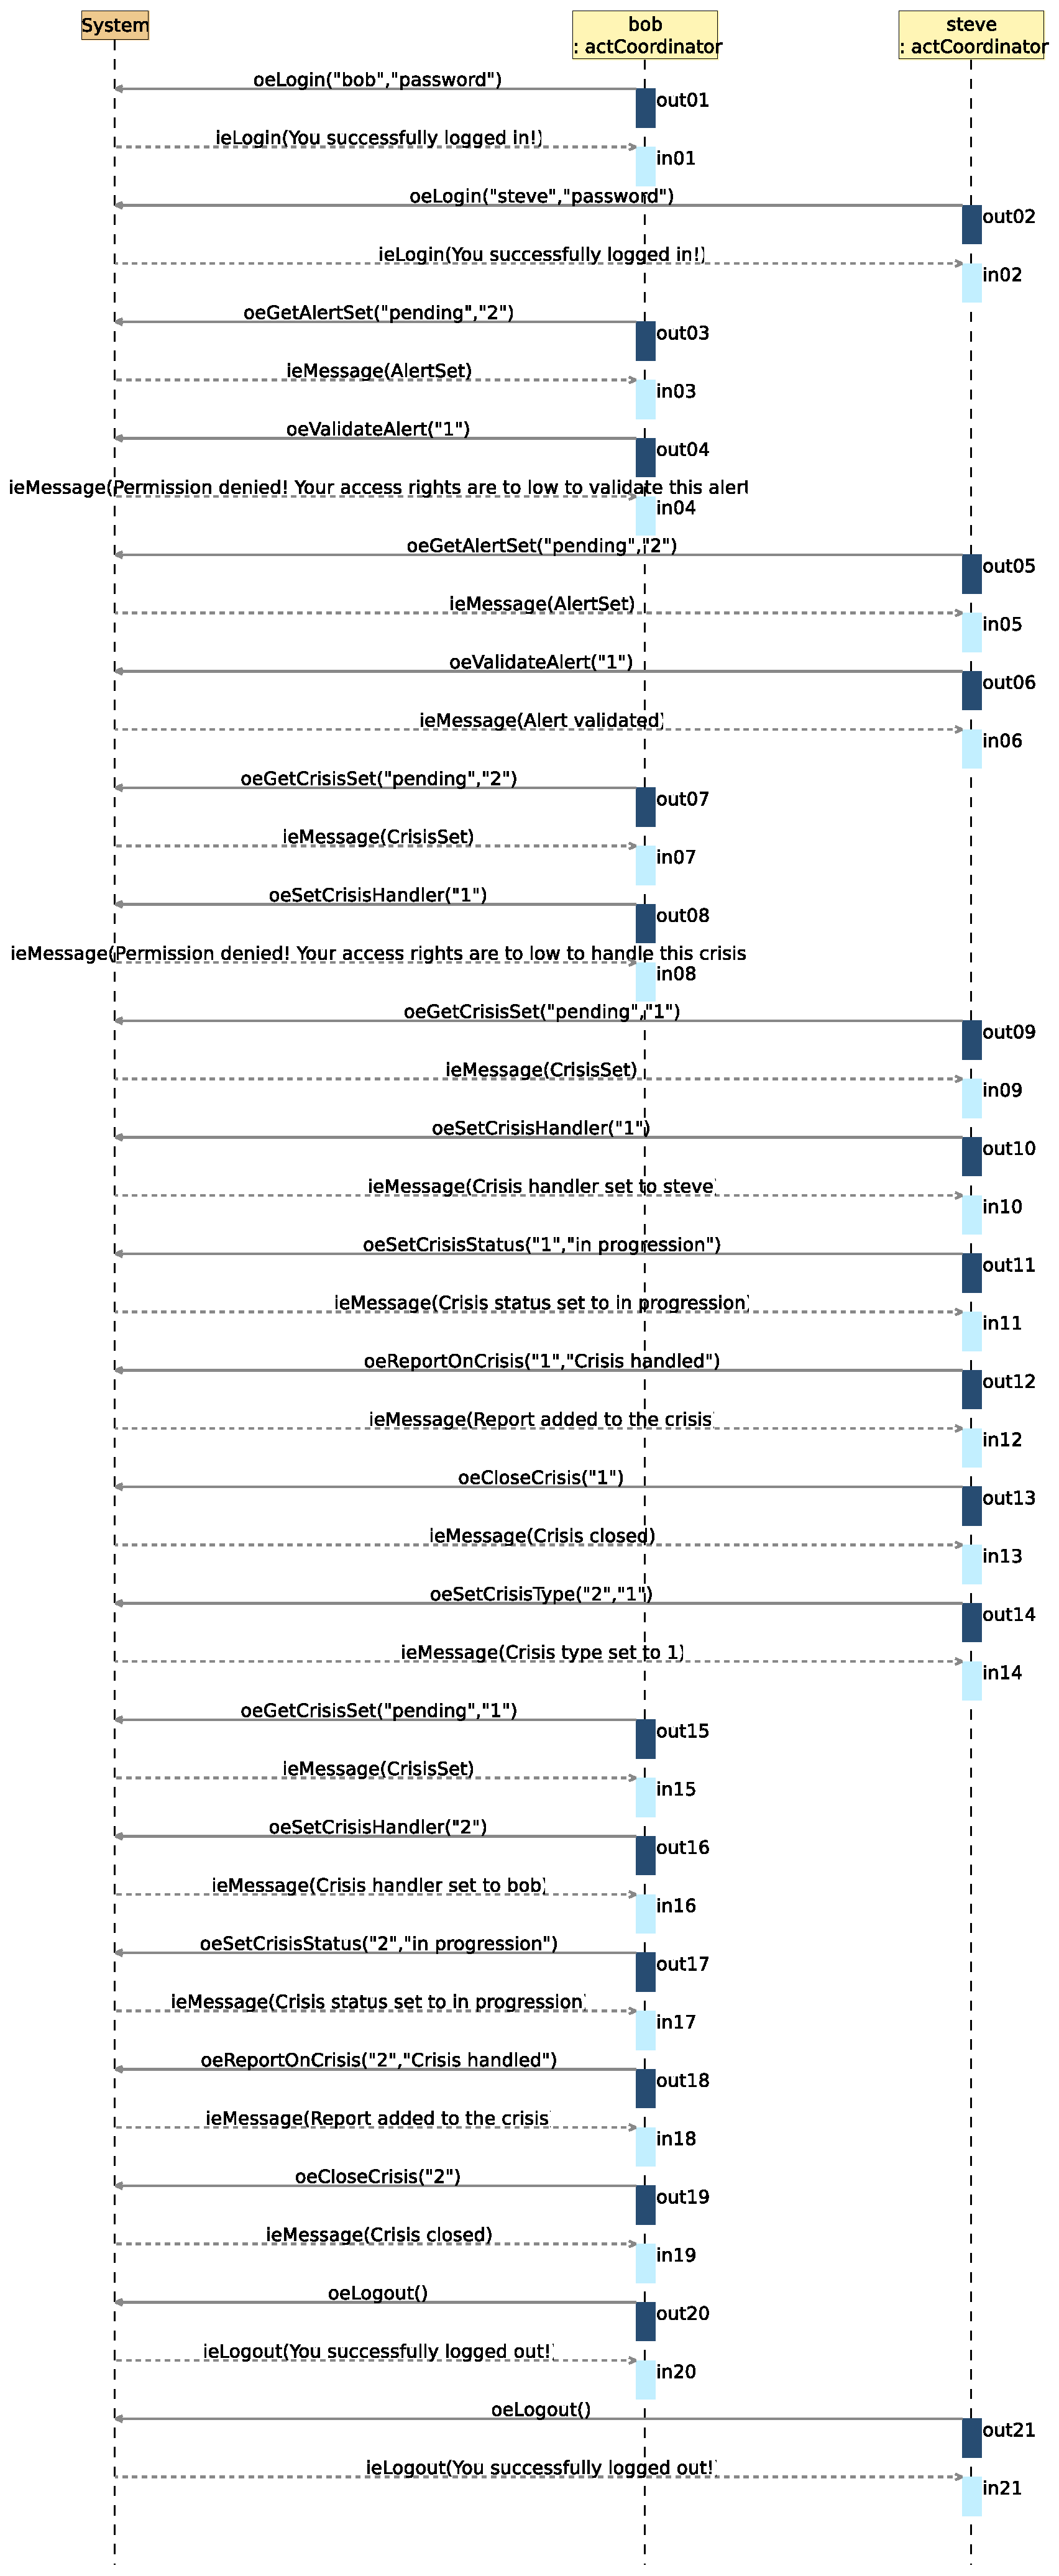
\includegraphics[
	angle=0
	,height=1.0\textheight
	]{./images-report-gen/usecase-model/summary/uci-ucisuGlobalCrisisHandling.eps}
	\end{center}
	\caption[lu.uni.lassy.excalibur.MyCrash.G02 Sequence Diagram: uci-ucisuGlobalCrisisHandling]{}
	\label{fig:lu.uni.lassy.excalibur.MyCrash.G02-RE-UC-uci-ucisuGlobalCrisisHandling}
	\end{figure}
	\vspace{0.5cm}
